\documentclass{mcmthesis}
\mcmsetup{CTeX = true,   % 使用 CTeX 套装时,设置为 true
        tcn = 0000, problem = B,
        sheet = true, titleinsheet = true, keywordsinsheet = true,
        titlepage = false, abstract = true}
\usepackage{palatino}
\usepackage{lipsum}
\title{The \LaTeX{} Template for MCM Version \MCMversion}
\author{\small \href{http://www.latexstudio.net/}
  {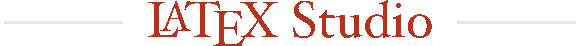
\includegraphics[width=7cm]{mcmthesis-logo}}}
\date{\today}
\begin{document}
\begin{abstract}
\lipsum[1]%写summary的地方
\begin{keywords}
keyword1; keyword2
\end{keywords}
\end{abstract}
\maketitle
\tableofcontents
\newpage

\section{Introduction}
\subsection{Background}

Lewis Mumford, a famous sociologist and literary critic,
once said in a metaphorical manner, ``Adding highway lanes
to deal with traffic congestion is like loosening your
belt to cure obesity.`` Fortunately, he did not experience
the worse congestion around today`s highway toll plaza.

Currently, with roaring number of vehicles, rising
construction costs and constrained available areas,
traffic jam becomes more and more serious but future
toll-plaza construction opportunities are limited to
improve this situation markedly. Figure 1 shows the
congestion in the toll plaza near Tappan Zee Bridge.

\begin{figure}[h]
\small
\centering
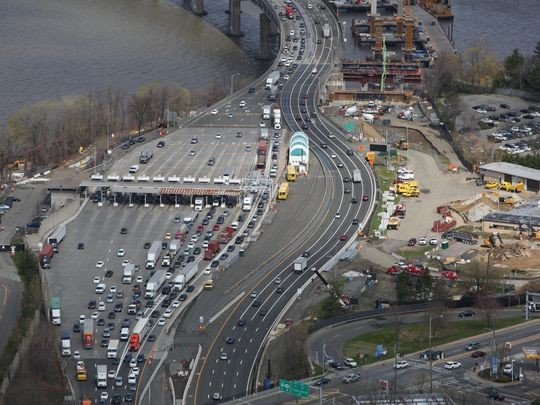
\includegraphics[width=10cm]{figure1}
\caption{Toll Plaza Congestion}\label{fig1}
\end{figure}

Subject to the constraints referred above, neither
increasing highway lanes nor building more tollbooths
seems practical enough to relieve traffic jam around a
toll plaza nowadays, particularly for some heavily-traveled
 roads such as the Garden State Parkway, New Jersey.
 Therefore, looking for some innovative design improvements
  on the geometric parameters of the extent toll plaza
  is an effective solution.


\subsection{Restatement of the Problem}
In this paper, we are required to explore if there is a
better-than-ever toll plaza model with specific shape,
size, and merging pattern. In this model, the prerequisite
is that vehicles fan in from $B$ tollbooth egress lanes down
to $L$ ($B\textgreater L$) lanes of traffic (i.e., the number of both
tollbooths and the lanes after merging are fixed). We aim
to construct a model that can optimize the arrangement
according to the following conditions.

\begin{itemize}
\item Enhance the capability of the accident prevention(A).
\item Maximize the throughput(T).
\item Minimize the cost of the land and road
construction(C).
\end{itemize}

Through our analysis, we determine if there are better
solutions than any toll plaza in common use. Afterwards,
the performance of our solution in light and heavy traffic
and other various situations along with corresponding
sensitivity analysis is discussed.

\subsection{Our Work}

\section{Assumptions}

\section{Notations}

\section{Model}
\subsection{Time Cost and Construction Cost}
\subsection{CA Model}

\section{Size}

The size of the merge area can be determined by
the following parameters:
\begin{itemize}
\item Total width of typical toll lanes ($W_{B}$).
\item Length of the recovery zone ($L_{r}$).
\item Length of total departure zone($L_{d}$).
\item Width of the exit($W_{L}$).
\end{itemize}
Parameters hereinbefore are shown in Figure \ref{fig4}.
\begin{figure}[h]
\small
\centering
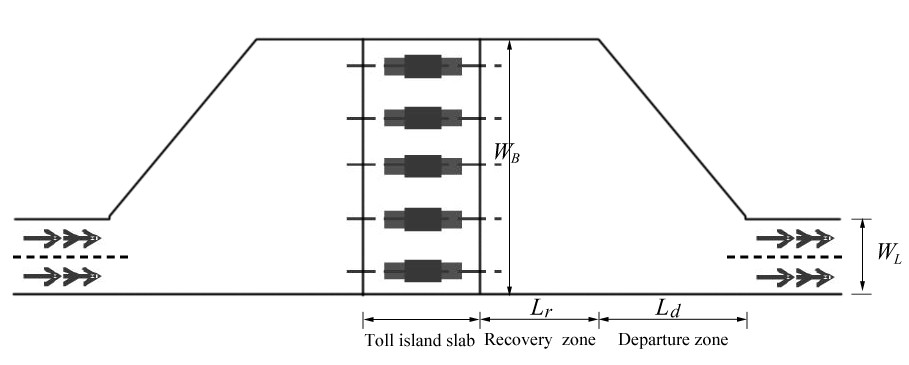
\includegraphics[width=10cm]{figure4}
\caption{The Parameters}\label{fig4}
\end{figure}
For the number of travel lanes ($L$) is fixed, $W_{L}$ is
constant. Then we are considering the effect of the
rest parameters separately. By simulating our model
mentioned above via computer program, we can figure
out how these parameters affect the maximal throughput
of the merge area, that is, $Q_{max}$.
Figure \ref{fig5} shows the variation tendency of
$Q_{max}$ with
the alteration of the width of each tollbooth $W_{b}$.
Apparently $W_{B} = B \times W_{b}$. Figure \ref{fig5}
provides a result
under the prerequisite that $W_b$ ranges from 6 to 14
while other parameters are fixed.
\begin{figure}[h]
\small
\centering
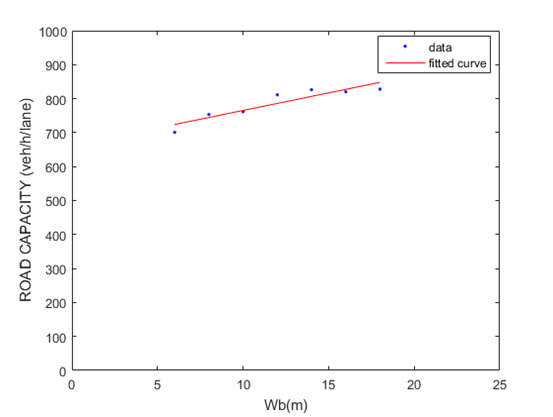
\includegraphics[width=10cm]{figure5}
\caption{The Linear Fitting Image of $Q_{max}$ and $W_b$}\label{fig5}
\end{figure}
We utilize an appropriate Linear Fitting Function Model
to address the data, and then get the fitting function
of $Q_{max}$ and $W_b$:
$$Q_{max}=p_{1}\times W_b+p_2$$
Where, $$p_1 =10.35, p_2 = 661.7$$
The simulation result indicates that $Q_{max}$ would only
be affected by the total width of typical toll lanes
($W_B$) in a small degree. However, increasing $W_b$ will
markedly result in a rise in construction costs.
For $L_r$, the linear fitting image is showed in Figure \ref{fig6}
and the variance of $Q_{max}$ is 36.7188. We can see that
$L_r$ causes almost no effect on the merge area capacity.
In the Linear Fitting Function, the coefficient $p_3=0$.
\begin{figure}[h]
\small
\centering
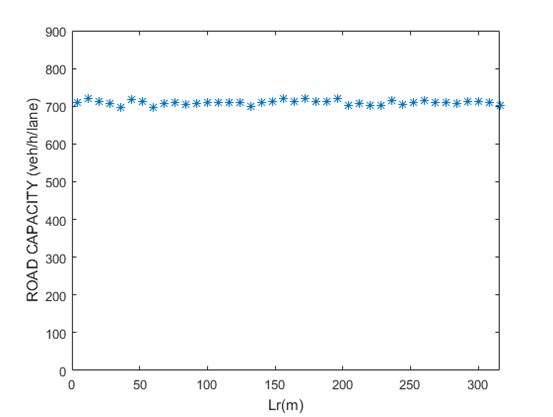
\includegraphics[width=10cm]{figure6}
\caption{The Linear Fitting Image of $Q_{max}$ and $L_r$}\label{fig6}
\end{figure}

Both linear fitting image, and function of $Q_{max}$ and
$L_d$ are shown below. There is a negative correlation
between $Q_{max}$ and $L_d$. Nevertheless, the relationship
is so faint that enlarging $Q_{max}$ by changing $L_d$ is
not functional.
\begin{figure}[h]
\small
\centering
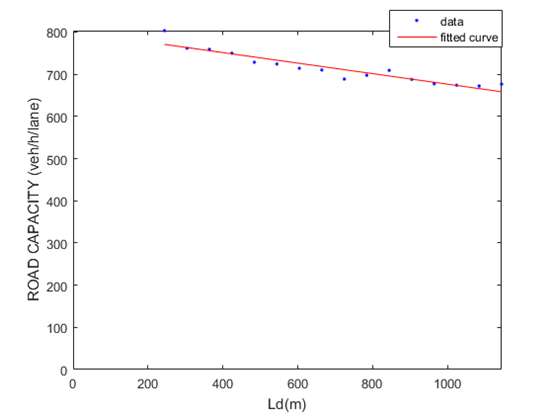
\includegraphics[width=10cm]{figure7}
\caption{The Linear Fitting Image of $Q_{max}$ and $L_d$}\label{fig7}
\end{figure}

$${Q_{3max}} = {p_5}\times {L_d} + {p_6}$$

Where, $$p_5 =-0.1248, p_6 = 801.1.$$
From discussion above, the size does cause impact on
$Q_{max}$, while the impact is not that obvious.
In addition, $L_d$ and $W_B$ should never be constructed
too small because it may cause potential safety
problems and result in higher accident rate.
For ensuring safety, the departure taper rates $T_r$
 must be limited into $[T_{rmin}, T_{rmax}]$. In summary,
 in order to determine the optimal size of a toll
 plaza, the problem can be transformed into a linear
 minimization problem with the form:

 \begin{equation*}
 \begin{split}
  {\bf minimize}\quad &$ $C$ = $S$($C_{road}$ + {$C_{construct}$}) + 4380$h_g^2${C_h}({Q_g} - {Q_{\max }})$\\
   {\bf s.t}\quad  & $$Q_{max}$|W_b = 3m, L_d = 612m, L_r = 168m = 709XL\\
       & \frac{dQ_{max}}{dW_{b}}=p_{1}=10.35\\
       & \frac{dQ_{max}}{dL_{r}}=p_{3}=0\\
       & \frac{dQ_{max}}{dL_{d}}=p_{5}=-0.1248\\
       & T_{rmin}\textless T_r\textless T_{rmax}\\
       & W_b\textgreater W_{bmin}\\
 \end{split}
 \end{equation*}

Here $W_{bmin}$ signifies the minimal width of the toothbooths, and
the area of toll plaza
$$S=13W_b(L_r+0.5L_d)+0.5LW_{L}L_{d}$$
The departure taper rate
$$T_r=\frac{L_d}{13W_b-LW_{L}}

For example, there is a toll plaza with three lanes
and eight tollbooths. To solve the problem, we can
make assumptions as following:
\begin{itemize}
\item The limited speed is 30 km/h.
\item The lifespan planned reaches to 10 years.
\item The average daily congestion time $h_g = 1h$.
\item The average congestion flow $Q_q=2300 veh/h$.
\item The land price locally $C_{land}=85 USD/m^2$
\item The cost of highway construction $C_{road}=357 USD/m_2$
\end{itemize}

According to \emph{1994 Green Book} taper rate for lane
addition in a 3-lane section ,$T_r$ should arrange from 8
to 15. Commonly, it takes 1 USD as the cost for each per
son to wait one hour.


On the basis of these conditions, the optimal solution of
linear programming is
\begin{align}
             W_b&=5   \\
             L_r&=47m \\
             L_d&=265.5m
\end{align}
the total cost  $$C=8,167,645USD$$


\section{Shape}

We propose two types of the plaza shape:
series type and parallel type.
\subsection{Series Type}
Literally, this type is to connect two or more merge
areas in series. Here, we only consider connecting
two merge areas. Furthermore, we might as well suppose
$B=8$ and $L=3$. Specially, vehicles fan in from eight
tollbooth egress lanes down to six lanes of traffic,
then fan in from six lanes of traffic to three, as
Figure \ref{fig8} shows.
\begin{figure}[h]
\small
\centering
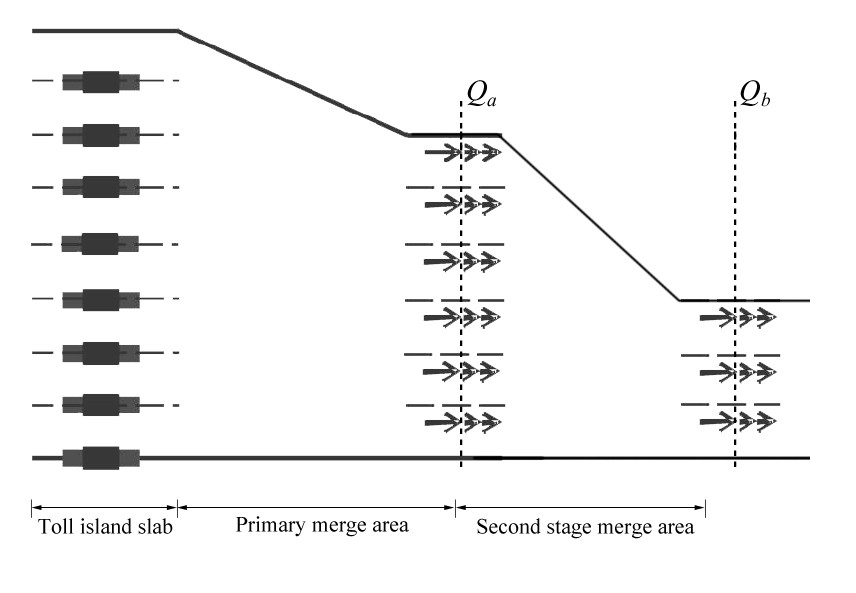
\includegraphics[width=10cm]{figure8}
\caption{Series Type}\label{fig8}
\end{figure}

According to the Buckets Effect (BE),
$$Q_{smax}=min⁡\left\{ Q_{amax},Q_{bmax} \right\}$$
$Q_{amax}$, $Q_{bmax}$ and $Q_{smax}$ respectively
signify the
maximal throughput of the primary merge area,
second stage merge area and the whole series-type
toll plaza.
We can get Table \ref{tab1} from simulation results, which
indicates the value of the maximal throughput for
each traffic line($Q_{emax}$) with different
$B$ and $L$ ($B\textgreater L$).
% Table generated by Excel2LaTeX from sheet 'Sheet1'
\begin{table}[htbp]
  \centering
  \caption{$Q_{max}$ with B and L}\label{tab1}
    \begin{tabular}{lllllllllll}
    \toprule
    $Q_{max}$     & B=1   & B=2   & B=3   & B=4   & B=5   & B=6   & B=7   & B=8   & B=9   & B=10 \\
    \midrule
    L=1   &       & 882   & 845   & 832   & 796   & 771   & 772   & 736   & 689   & 640 \\
    L=2   &       &       & 815   & 789   & 773   & 755   & 720   & 718   & 686   & 659 \\
    L=3   &       &       &       & 755   & 758   & 734   & 724   & 709   & 684   & 671 \\
    L=4   &       &       &       &       & 724   & 700   & 715   & 695   & 694   & 673 \\
    L=5   &       &       &       &       &       & 716   & 695   & 690   & 688   & 673 \\
    L=6   &       &       &       &       &       &       & 695   & 688   & 682   & 667 \\
    L=7   &       &       &       &       &       &       &       & 682   & 676   & 670 \\
    L=8   &       &       &       &       &       &       &       &       & 676   & 660 \\
    L=9   &       &       &       &       &       &       &       &       &       & 651 \\
    \bottomrule
    \end{tabular}%
  \label{tab:addlabel}%
\end{table}%

As for the example shown in Figure \ref{fig8},
$$Q_{smax}=min⁡\left\{ 688\times6,734\times3 \right\}$$
For a simple toll plaza with the same number of B and L,
$$Q_{max}=709\times3=2127$$
Therefore
$$Q_{smax}>Q_{max}$$
Moreover, since $Q_{emax}$ is becoming large as $B$ or $L$ d
ecrease, we can prove that the merge area in series
type would have a larger capacity for any $B$ and $L$ ($B\textmore L$).
Thus, connecting two or more merge area in series is a
practical and optimized scheme.


\subsection{Parallel Type}
That is, divide the merge area transversely and put
them together in parallel. Similarly, if we suppose
$B=8$ and $L=3$ again, the toll plaza can be divided into
two portions as Figure \ref{fig9} shows.
\begin{figure}[h]
\small
\centering
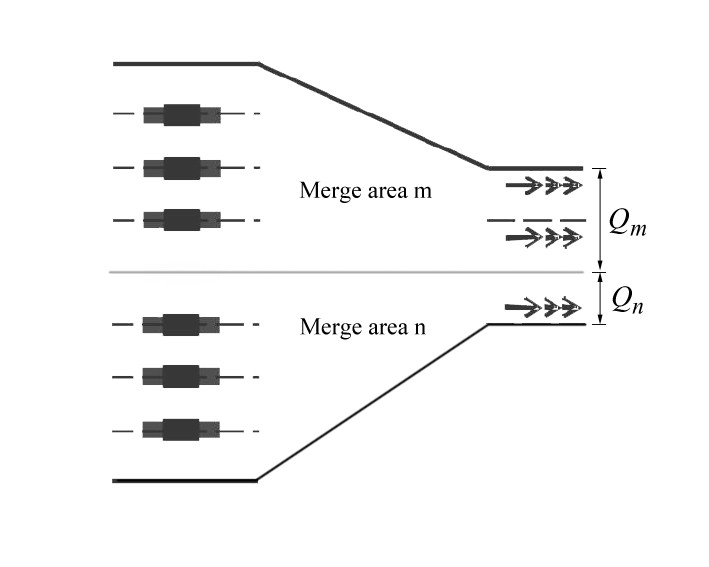
\includegraphics[width=10cm]{figure9}
\caption{Parallel Type}\label{fig9}
\end{figure}
Since the two areas are juxtaposed,
$$Q_{pmax}=Q_{mmax}+Q_{nmax}$$
$Q_{mmax}$, $Q_{nmax}$ and $Q_{pmax}$ respectively
signify the maximal throughput of the merge area m,
merge area n and the whole parallel-type toll plaza.
Similar to the analysis of the series type,
$Q_{emax}$ is becoming large with the increasing
of $B$ or $L$. Thus, this solution could enlarge
the maximal throughput efficaciously.

\subsection{An example}
For the convenience of discussion, we still take a
toll plaza with three lanes and eight tollbooths
as an example. If we adopt the method of 8-6-3 series
type, from what has been discussed above, $Q_{max}$
increases from 2127 to 2212 veh/h with increasing
rate of 3.9\%. Therefore, the cost time decreases
 by 1.4\%.


However, at the same time, the area $S_r$ and $S_d$
increases. The total area will increase by
$$\Delta S=4W_{b}L_{d}+W_{L}(6L_r+3L_d)$$
We can solve out that the total area will
increase by 73.4\%.Thus, the construction cost will
also increase by 73.4\%. Under normal conditions
, construction cost and time cost are of the
same order of magnitude, so the series cannot
solve the problem practically.

On the other hand, if we adopt the method
of parallel type ,we can find that Qmax
increase by 13.3\%, which is fully significant.
And we adopt the structure shown in figure X
simultaneously. Such shape would cause the total
area to increase by the following formula:
$$\Delta S=6W_{L}(L_D+L_r+L_A)$$
Where $L_{A}$ is the length of approving zone of
the toll plaza, which increases by 21.3\% approximately. Hence it is necessary to construct
toll plaza in this way when the traffic congestion
is serious and the cost time is extremely large.


\section{Merging Pattern}

Here, we devise a real-time merging control system for
toll plaza based on the previous work by M. Papageorgiou
et al. Through our improvement, it can be specially used
for the toll plaza we are discussing. In addition, this
system can effectively maximize the throughput by
maintaining the occupancy of departure area close to a
critical value. Figure \ref{fig2} illustrates the framework of
this system.

\begin{figure}[h]
\small
\centering
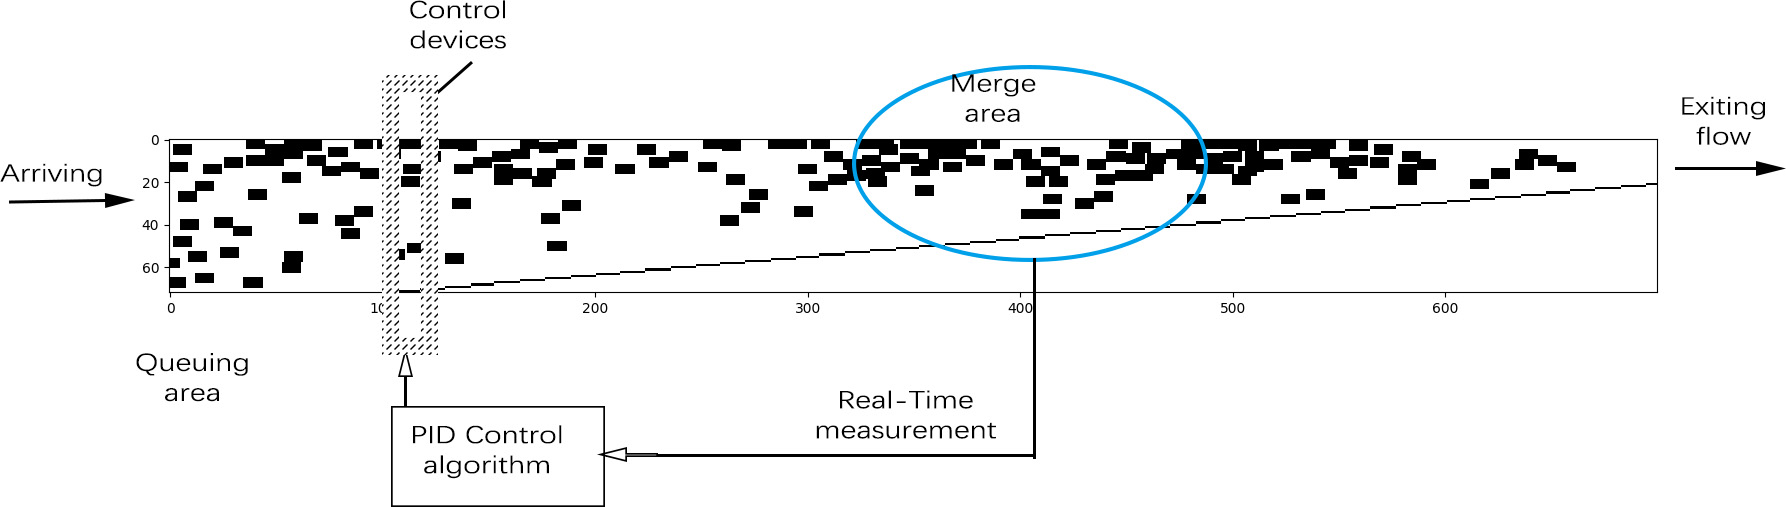
\includegraphics[width=10cm]{figure2}
\caption{The Framework of This System}\label{fig2}
\end{figure}
%此处的figure被放到了下一页



\textbf{Merge area}

As a matter of fact, the merge area is equal to the
departure zone as referred to above. Typically, it
is an approximately trapezoidal area where the vehicles
leave from the booths on a total of $B$ lanes and finally
fit into $L$ lanes of the exit. Here, we focus on the
flow-density variation with the occupancy increasing
in the merge area. Eventually,according to our CA
model's simulation, we obtain a diagram to
describe this functionary relationship, which is shown
in Figure \ref{fig3}.

\begin{figure}[h]
\small
\centering
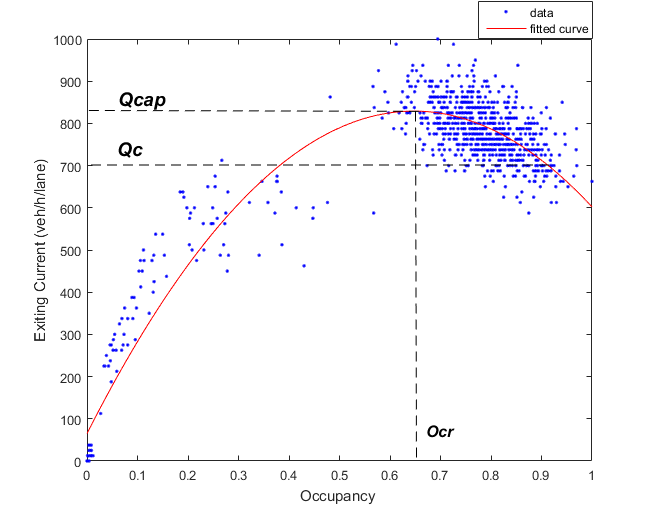
\includegraphics[width=10cm]{figure3}
\caption{The Functionary Relationship}\label{fig3}
\end{figure}

After noticing that X-axis is occupancy $o$ (\%), while
Y-axis represents the exit flow $q_{out}$, we can tell from
the diagram:
\begin{itemize}
\item When $o$ is small, merging conflicts are scarce.
the exit flow is correspondingly low and it
 increases linearly with density increasing
\item As $o$ increases, merging conflicts may increase, but
$q_{out}$ also increases as well until, for a specific value
$o_{cr}$, the exit flow reaches the capacity $q_{cap}$.
\item If $o$ increases beyond $o_{cr}$, merging conflicts
become more frequent, leading to a serious congestion.
Consequently, a capacity drop happens.
\end{itemize}
Therefore, we can conclude that the occupancy of the merge
area can directly influence the exit flow, or rather, the
throughput. And we can regulate the occupancy under the
goal to maintain $o  \approx  o_{cr}$ by controlling the merging
pattern with the assistant of a control algorithm and
feedback. From a macroscopic perspective, the maximum
throughput can be achieved by a certain merging pattern
design. As a result, our goal is to model this design.

\textbf{Feedback control based on PID controller}

We are inspired by the commonly used PID control algorithm in industrial
control systems and
decide to deploy traffic lights to individual lanes
as control devices.


However, the most crucial task is to determine the
form of feedback control.

Our goal is to ensure that occupancy is maintained
at around $o_{cr}$ regardless of how serious the traffic congestion is.
What's different from common PID control system is that the traffic
system is not a Continuous system,and
The control loops are very long compared to other systems.
We suppose that the feedback control is activated
at each discrete time interval witch usually set as 1~2 min. After activation, it
will collect latest measurements of occupancy $o$, and
send data-converted instructions to control devices
under the purpose of maintaining $o  \approx  o_{cr}$.


The PID system can be expressed as:

  \[q\left( n \right) = K_{p}e\left( {n - 1} \right) + {K_i}\sum_{j=1}^{n-1} e\left( {n - 1} \right)+\frac{d}{dx} \left[ e\left( {n - 1} \right)-e\left( {n - 2} \right)\right]
  \]
  \[
  e\left( {n} \right)=\hat{o}\left( {n} \right)-o\left( {n} \right)
  \]
Where,

% Table generated by Excel2LaTeX from sheet 'Sheet1'
\begin{table}[htbp]
  \centering
    \begin{tabular}{ll}
      \toprule
    $n$     & The discrete time index \\
    $q(n)$  & The controlled entering flow (veh/h) to be implemented in a new time step $n$ \\

    $o(n)$ & The measured occupancy of merge area in this time step \\
    $\hat{o}$ & The desired value of occupancy (can be set as $o_{cr}$) \\
    $K_{p},K_i,K_d$  & coefficients for the proportional, integral, and derivative terms, always positive \\
    \bottomrule
    \end{tabular}%
  \label{tab:addlabel}%
\end{table}%

In addition, the occupancy measurement should best be
placed at or just upstream of the location where serious
vehicle decelerations (congestion) appear first.

\section{Conclusion}

\section{Sensitivity Analysis}
\subsection{The Performance of Our Solution in Light
and Heavy Traffic}
\subsection{Autonomous Vehicles}
\subsection{The Proportions of Different Tollbooths}

\section{Strengths and Weaknesses}
\subsection{Strengths}
\subsection{Weaknesses}

\begin{thebibliography}{99}
\bibitem{1} D. E. KNUTH   The \TeX{}book  the American
Mathematical Society and Addison-Wesley
Publishing Company , 1984-1986.
\bibitem{2}Lamport, Leslie,  \LaTeX{}: `` A Document Preparation System '',
Addison-Wesley Publishing Company, 1986.

\end{thebibliography}

\begin{appendices}

\section{First appendix}


Here are simulation programmes we used in our model as follow.\\

\textbf{\textcolor[rgb]{0.98,0.00,0.00}{Input matlab source:}}
\lstinputlisting[language=Matlab]{./code/mcmthesis-matlab1.m}

\section{Second appendix}

some more text \textcolor[rgb]{0.98,0.00,0.00}{\textbf{Input C++ source:}}
\lstinputlisting[language=C++]{./code/mcmthesis-sudoku.cpp}

\end{appendices}
\end{document}

%%
%% This work consists of these files mcmthesis.dtx,
%%                                   figures/ and
%%                                   code/,
%% and the derived files             mcmthesis.cls,
%%                                   mcmthesis-demo.tex,
%%                                   README,
%%                                   LICENSE,
%%                                   mcmthesis.pdf and
%%                                   mcmthesis-demo.pdf.
%%
%% End of file `mcmthesis-demo.tex'.
